\section{Przegląd istniejących rozwiązań}

%------------------------------------------------

\begin{frame}
\frametitle{Robot Velma}
\begin{figure}
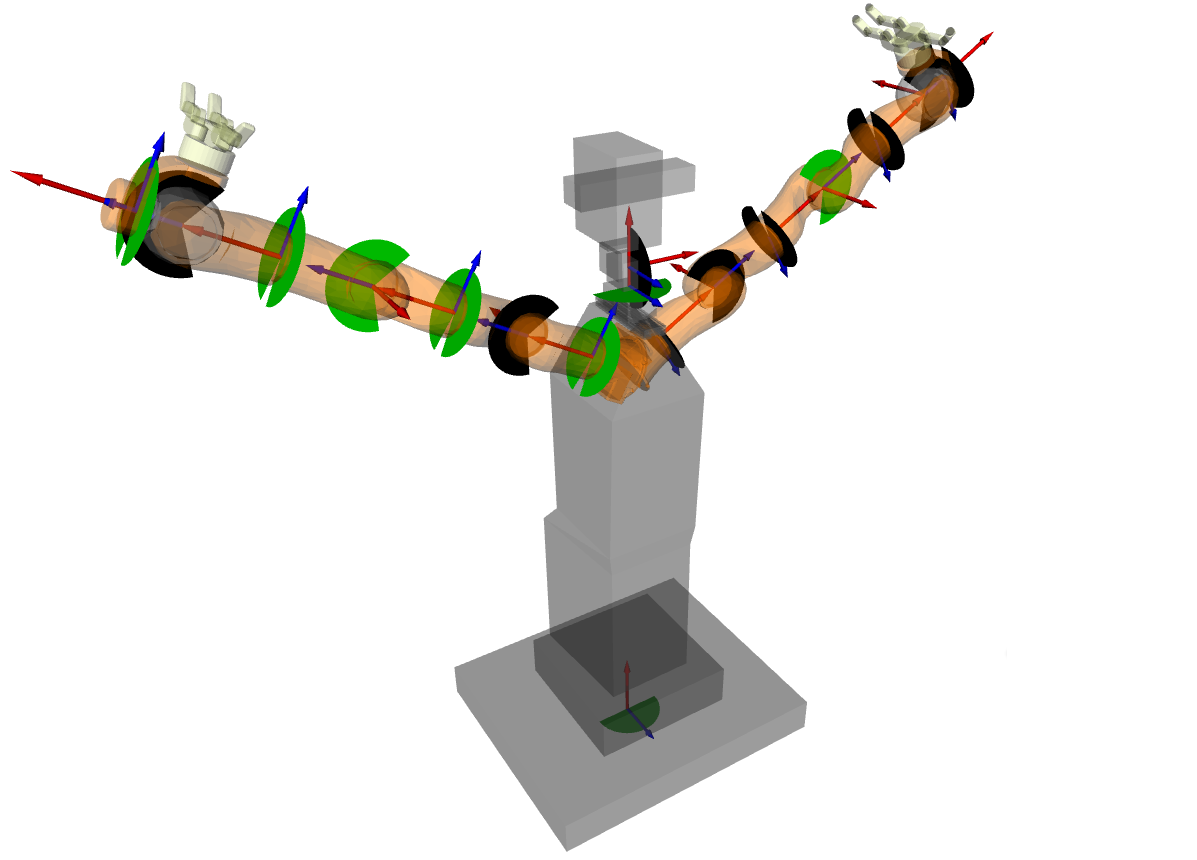
\includegraphics[scale=0.22]{./images/velma_joints.png}
\setcaptioncitation{\texttt{https://rcprg-ros-pkg.github.io/velma\_docs/2017/10/13/01/01\_{}introduction\_{}02\_{}velma\_{}robot/}}
\caption{Wizualizacja robota Velma z zaznaczonymi stopniami swobody \cite{docsVelma}}
\end{figure}
\end{frame}

%------------------------------------------------

\begin{frame}
\frametitle{Robot Velma}
\begin{figure}
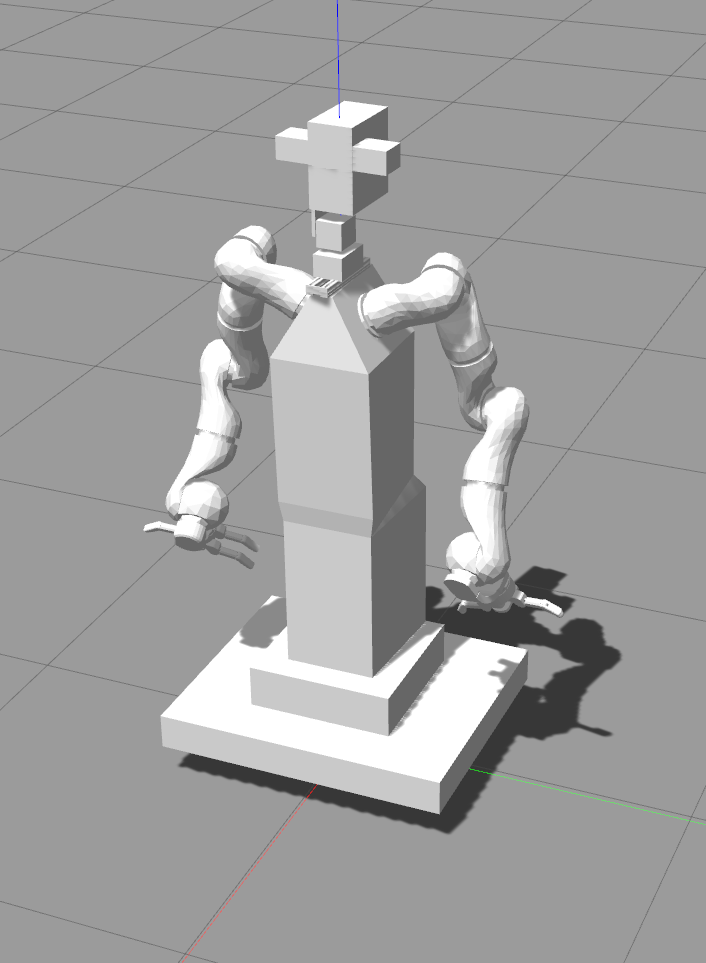
\includegraphics[scale=0.20]{./images/velma_gz_cropped.png}
\caption{Robot Velma w symulatorze Gazebo}
\end{figure}
\end{frame}

%------------------------------------------------

\begin{frame}
\frametitle{Robot Velma}
Robot Velma składa się z \cite{docsVelma}:  
\begin{itemize}
	\item obrotowego korpusu
	\item dwóch manipulatorów KUKA LWR
	\item dwóch chwytaków BarrettHand
	\item szyi o dwóch stopniach swobody
	\item kamery Kinect XBOX 360
\end{itemize}
\end{frame}

%------------------------------------------------

\begin{frame}
\frametitle{Struktura symulatora}

\end{frame}

%------------------------------------------------

\begin{frame}
\frametitle{Robot Velmobil}
\begin{figure}
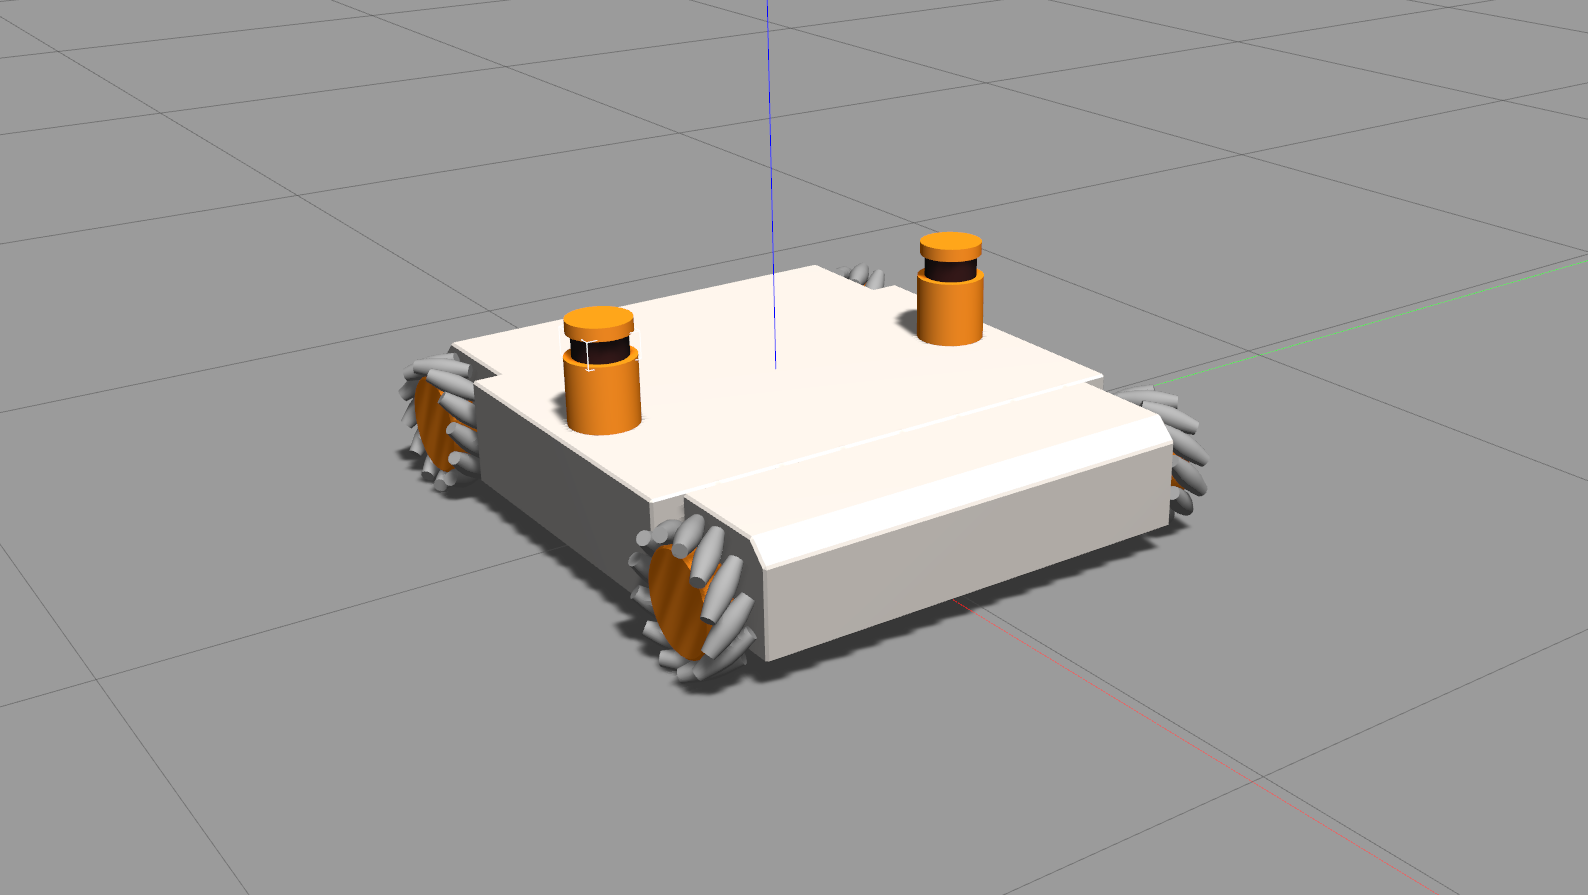
\includegraphics[scale=0.20]{./images/omnivelma_gz.png}
\caption{Baza mobilna robota w symulatorze Gazebo}
\end{figure}
\end{frame}

%------------------------------------------------

\begin{frame}
\frametitle{Robot Velmobil}
Robot Velmobil posiada \cite{docsVelma}:  
\begin{itemize}
	\item 4 koła szwedzkie
	\item dwa skanery laserowe LIDAR
	\item jednostkę inercyjną
	\item enkodery % jakie enkodery
\end{itemize}
\end{frame}

%------------------------------------------------

\begin{frame}
\frametitle{Struktura symulatora}

\end{frame}